\documentclass[main]{subfiles}
\begin{document}

\section*{Lecture 1 // Aug 25 // Overview}
\addcontentsline{toc}{section}{Lecture 1 -- Overview}

\begin{theorem}[Freedman]
Let $Q$ be a unimodular symmetric bilinear form. Then there exists a unique simply connected topological $4$-manifold $X^4$ such that $Q_X = Q$.
\begin{enumerate}
\item If $Q$ is even, there exists a unique smooth $X^4$ up to homeomorphism.
\item If $Q$ is odd, there exist at most two smooth $X^4$ up to homeomorphism, of which at most one is smoothable.
\end{enumerate}
\end{theorem}

\begin{theorem}[Donaldson]\label{thm:donaldson}
If $X^4$ is a simply connected, smooth, closed $4$-manifold and $Q_X$ is definite, then $Q_X$ is equivalent to $n\langle +1\rangle$ or $n\langle -1\rangle$.
\end{theorem}

\begin{example}
$E_8$ matrix:
\begin{center}
\begin{minipage}[t]{0.45\textwidth}
\centering
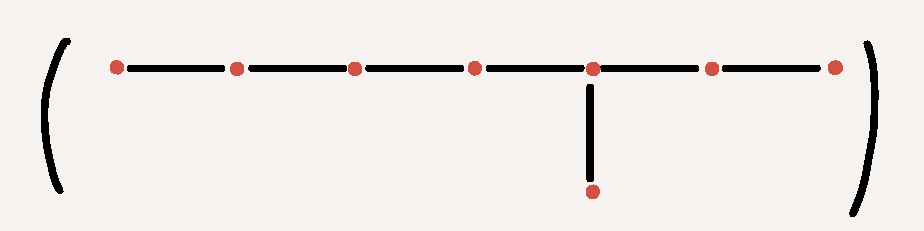
\includegraphics[width=0.9\linewidth]{figures/fig_lec1_e8_graph.png}
\end{minipage}%
\begin{minipage}[t]{0.5\textwidth}
\[
\mathrm{adj} = \begin{pmatrix}
-2 & 1 & 0 & 0 & 0 & 0 & 0 & 0\\
1 & -2 & 1 & 0 & 0 & 0 & 0 & 0\\
0 & 1 & -2 & 1 & 0 & 0 & 0 & 0\\
0 & 0 & 1 & -2 & 1 & 0 & 0 & 0\\
0 & 0 & 0 & 1 & -2 & 1 & 0 & 1\\
0 & 0 & 0 & 0 & 1 & -2 & 1 & 0\\
0 & 0 & 0 & 0 & 0 & 1 & -2 & 1\\
0 & 0 & 0 & 0 & 1 & 0 & 1 & -2
\end{pmatrix}
\]
\end{minipage}
\end{center}
Check: no change of basis takes this to $\pm I_8$.

\medskip
$\Rightarrow$ $E_8$ is realized by a non-smoothable topological $X^4$.

$\Rightarrow$ the same holds for $nE_8$.
\end{example}

Over the next few weeks, we'll discuss the proof of Donaldson's theorem. After, we'll discuss Instanton Floer Homology (IFH) and some applications to three-manifolds, in particular, the homology cobordism group. The rest of this lecture will be to lay the groundwork for this.

\subsection*{3-Manifolds}

\begin{definition}[Homology Cobordism Group]
\[
\Theta^3_{\mathbb{Z}} = \{\text{all } \mathbb{Z}\mathrm{HS}^3\text{'s}\}/\text{homology cobordism}.
\]
$Y_1 \sim Y_2$ are homology cobordant if there exists $W^4$, a homology $S^3\times I$, such that $\partial W^4 \cong -Y_1 \sqcup Y_2$.
\end{definition}

\begin{itemize}
\item The topological version is trivial.
\end{itemize}

\begin{theorem}[Freedman]
If $Y$ is a $\mathbb{Z}\mathrm{HS}^3$, then $Y=\partial W$ for some $\mathbb{Z}\mathrm{HB}^4$. In fact, $\pi_1 W = 1$.
\end{theorem}

\begin{proof}
Given a unimodular symmetric bilinear pairing $Q$, we can construct a smooth $X^4$ with boundary and intersection form $Q$ by attaching $2$-handles to $B^4$ according to $Q$:
\begin{center}
$E_8$:
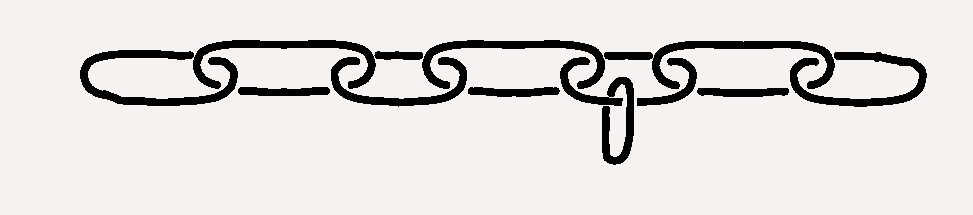
\includegraphics[width=0.5\linewidth]{figures/fig_lec1_e8_chain.png}
\end{center}

For $E_8$, $\partial E_8 \cong$ Poincar\'e homology sphere $\cong \Sigma(2,3,5)$.

By Donaldson, $\Sigma(2,3,5)$ does not bound any smooth $\mathbb{Z}\mathrm{HB}^4$
\[
\Rightarrow [\Sigma(2,3,5)] \neq 1 \in \Theta^3_{\mathbb{Z}}.
\]

Proof of boundary-diffeomorphism $\Sigma(2,3,5)\cong \partial E_8$:
\begin{center}
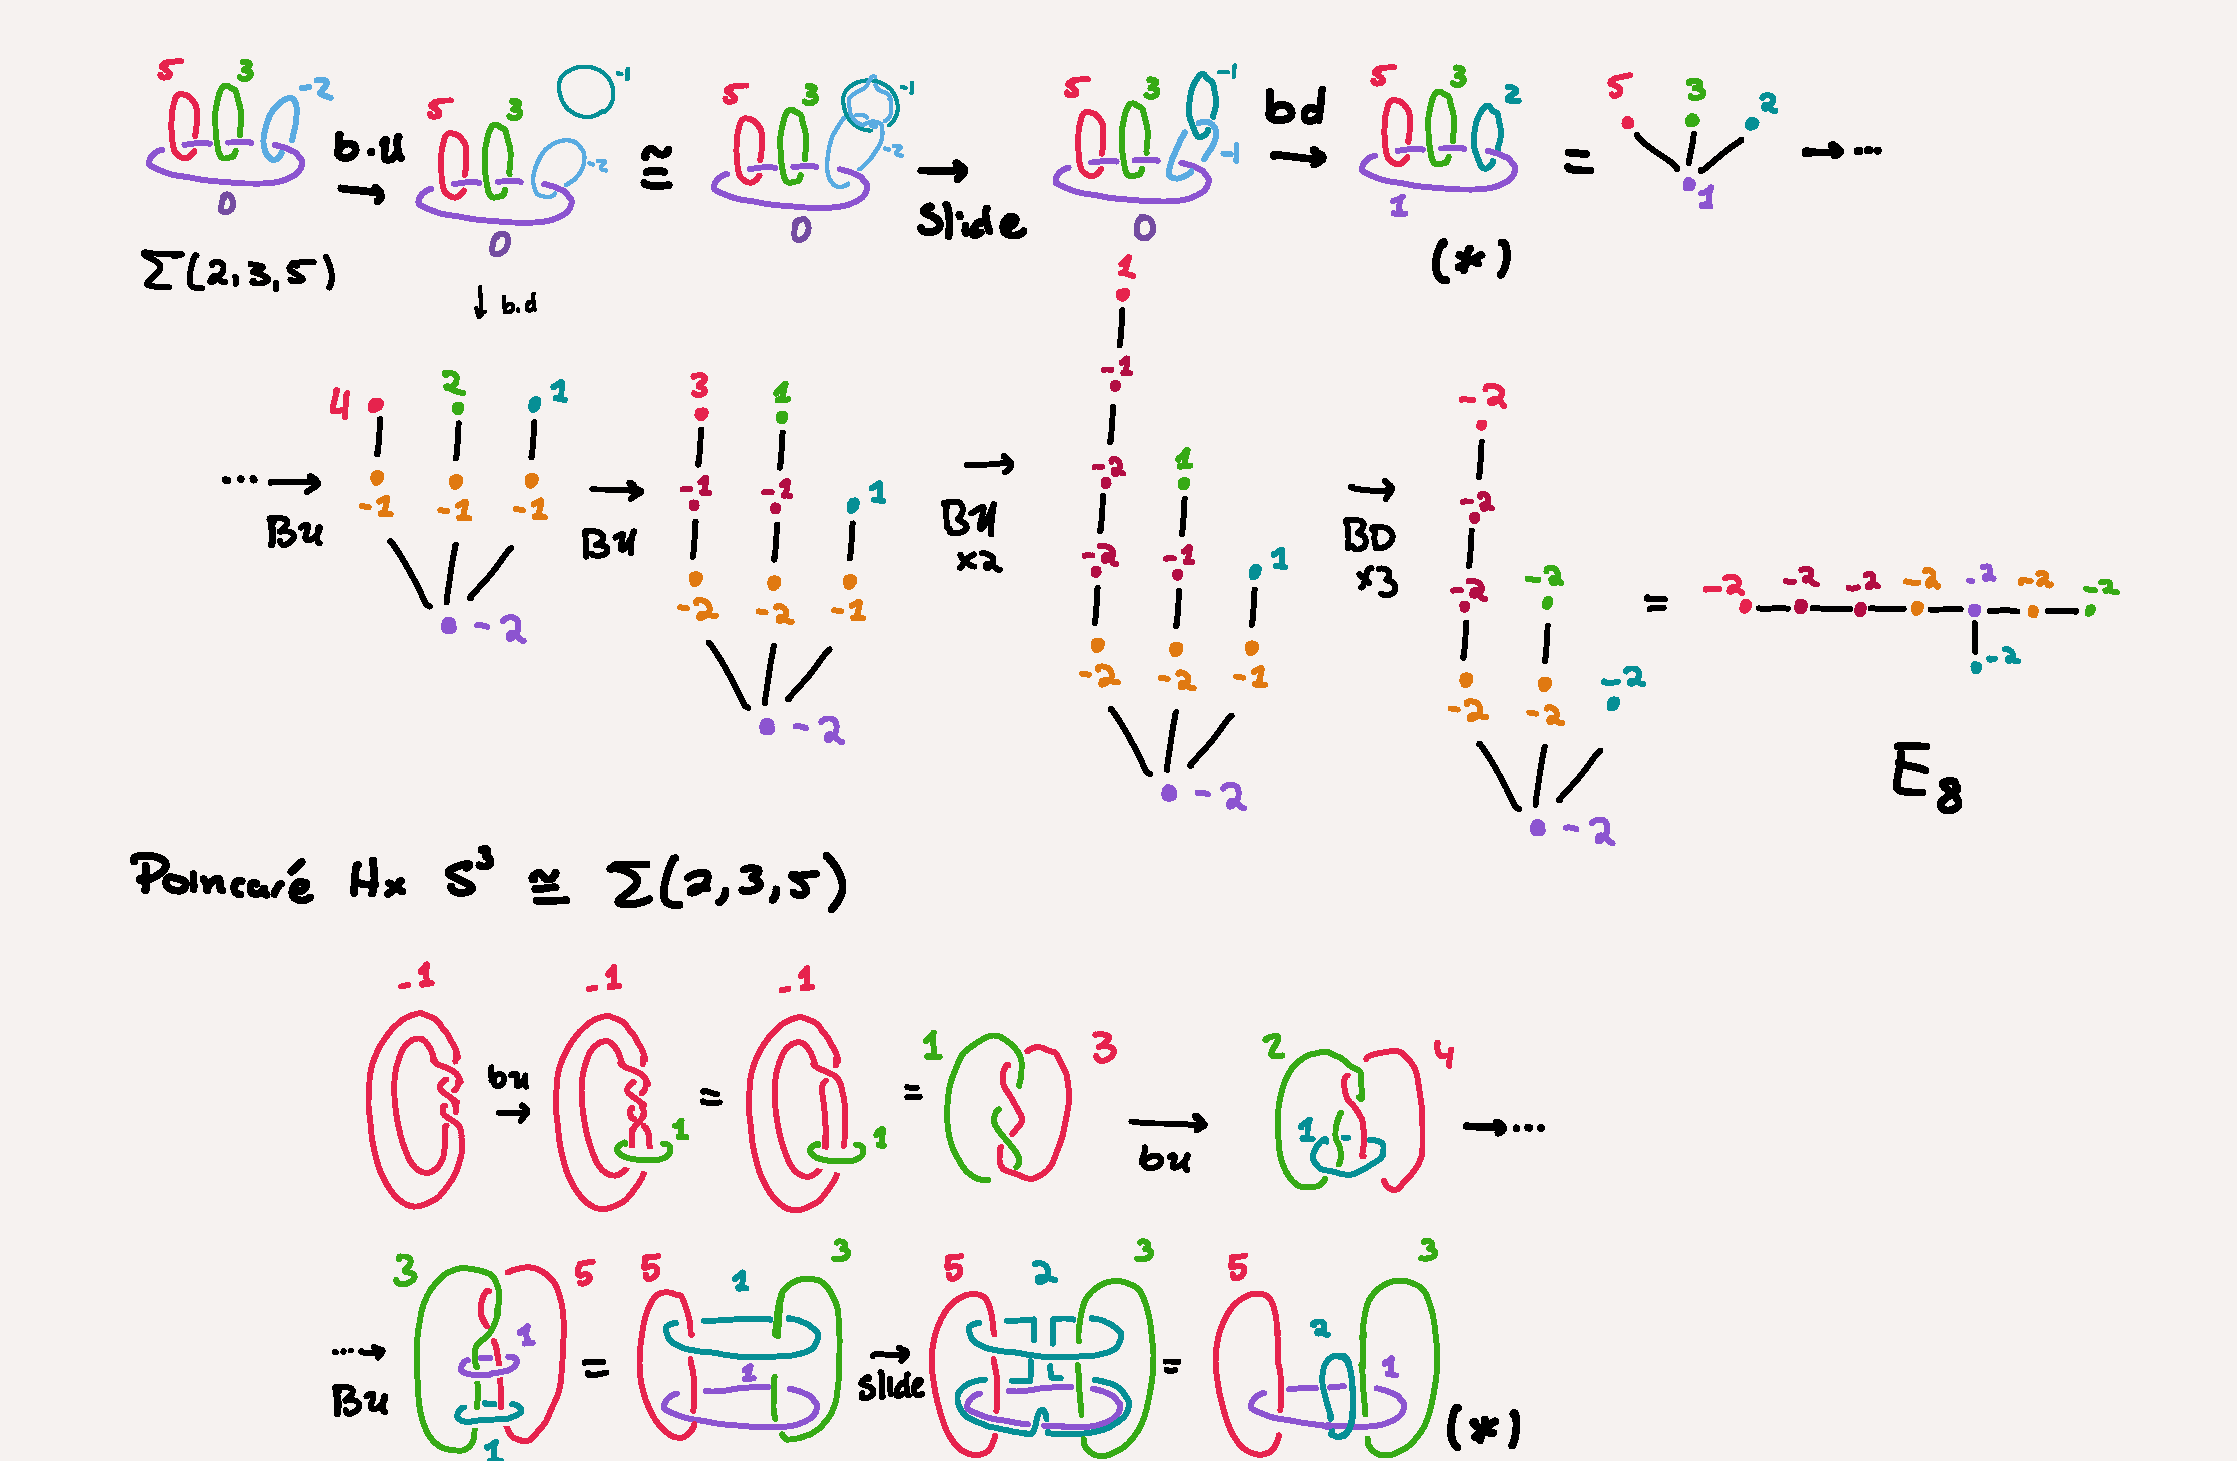
\includegraphics[width=\linewidth]{figures/fig_lec1_bdiffeo_proof.png}
\end{center}
\end{proof}

\begin{remark}
There are many $\mathbb{Z}\mathrm{HS}^3$'s.
\end{remark}

\begin{example}
Brieskorn spheres: $p,q,r$ pairwise coprime,
\[
\Sigma(p,q,r) := S^5_\epsilon \cap \{x^p+y^q+z^r=0\}\subseteq \mathbb{C}^6.
\]
\end{example}

\begin{example}
$S^3_{1/n}(k)$ for all $k$.
\end{example}

\begin{example}
Mazur manifolds: $1$-handle $\cup$ $2$-handle such that the algebraic linking is $\pm 1$, but the geometric linking is $\neq \pm 1$.
\end{example}

\begin{center}
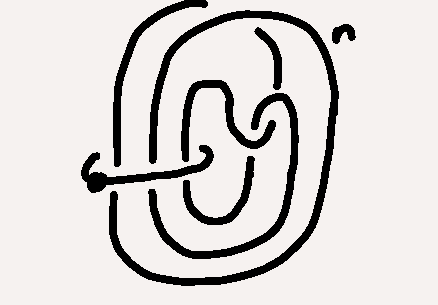
\includegraphics[width=0.22\linewidth]{figures/fig_lec1_framed_knot.png}
\end{center}

\begin{question}
How large is $\Theta^3_{\mathbb{Z}}$?
\end{question}

\begin{theorem}[Furuta, FS]
$\{\Sigma(2,3,6n-1)\}$ is a $\mathbb{Z}^\infty$ subgroup of $\Theta^3_{\mathbb{Z}}$.
\end{theorem}

\begin{theorem}[Daemi--Nozaki--Sato--Taniguchi]
Sometimes $\{S^3_{1/n}(k)\}$ are linearly independent.
\end{theorem}
This relies on a specific condition on $\mathrm{IFH}_\ast$.

\begin{note}
$\Sigma(2,3,6n-1) = S^3_{1/n}(T_{2,3})$.
\end{note}

From concordance to homology cobordism:
\[
\Sigma_2 : \mathcal{C} \longrightarrow \Theta^3_{\mathbb{Z}/2}, \qquad k \longmapsto \Sigma_2(k) = \text{double branched cover over } k,
\]
is a homomorphism.

\begin{question}
Is there a distinction between bounding a $\mathbb{Z}\mathrm{HB}^4$ and a $\pi_1=0$ $\mathbb{Z}\mathrm{HB}^4$? I.e., is there a $\pi_1=1$ homology cobordism from $\Sigma(2,3,5)$ to itself?
\end{question}

\begin{theorem}[Taubes]
No.
\end{theorem}

\begin{theorem}[Daemi--Nozaki--Sato--Taniguchi]
Often, no. Cutting open the cobordism, we get a simply connected $\mathbb{Z}\mathrm{HB}^4$ bounding $Y \# -Y$.
\end{theorem}

\end{document}
